\documentclass[a4paper, 12pt]{article}

\usepackage[utf8]{inputenc}
\usepackage[spanish]{babel}
\usepackage[margin=2cm]{geometry}
\usepackage{graphicx}
\usepackage{float}
\usepackage{pdfpages}
\usepackage{listings}
\usepackage{listingsutf8} % Incorpora acentos en los listings
\usepackage{xcolor}

\definecolor{mGreen}{rgb}{0,0.6,0}
\definecolor{mGray}{rgb}{0.5,0.5,0.5}
\definecolor{mPurple}{rgb}{0.58,0,0.82}
\definecolor{backgroundColour}{rgb}{0.95,0.95,0.92}

\lstset{
language=C,
%backgroundcolor=\color{backgroundColour},   
commentstyle=\color{mGreen},
%keywordstyle=\color{magenta},
keywordstyle=\color{blue},
%numberstyle=\tiny\color{mGray},
stringstyle=\color{mPurple},
tabsize=4,
basicstyle=\fontsize{11}{13}\ttfamily\footnotesize,
showspaces=false,
showstringspaces=false,
captionpos=b,
breaklines=true
}


%\lstdefinestyle{CStyle}{
%    backgroundcolor=\color{backgroundColour},   
%    commentstyle=\color{mGreen},
%    keywordstyle=\color{magenta},
%    numberstyle=\tiny\color{mGray},
%    stringstyle=\color{mPurple},
%    basicstyle=\footnotesize,
%    breakatwhitespace=false,         
%    breaklines=true,                 
%    captionpos=b,                    
%    keepspaces=true,                 
%    numbers=left,                    
%    numbersep=5pt,                  
%    showspaces=false,                
%    showstringspaces=false,
%    showtabs=false,                  
%    tabsize=2,
%    language=C
%}


\title{		\textbf{Trabajo Práctico 1}\\
			\textbf{Conjunto de instrucciones MIPS}
			}

\author{	Lucas Medrano, \textit{Padrón Nro. 00.000}                     	\\
            \texttt{ dirección de e-mail }                           		\\
            Federico Álvarez, \textit{Padrón Nro. 00.000}                 	\\
            \texttt{ dirección de e-mail }                                 	\\
            Facundo Fernández, \textit{Padrón Nro. 89.843}              	\\
            \texttt{ ffelfis@gmail.com}                                   	\\[2.5ex]
            \normalsize{Grupo Nro. \quad - 2do. Cuatrimestre de 2018}      	\\
            \normalsize{66.20 Organización de Computadoras}               	\\
            \normalsize{Facultad de Ingeniería, Universidad de Buenos Aires}\\
       }
\date{}

\begin{document}
	\lstset{inputencoding=utf8/latin1} % Incorpora acentos en los listings
	\maketitle
	\thispagestyle{empty}
	\begin{abstract}
		En este trabajo se quiere desarrollar un programa escrito en lenguaje C que implementa un algoritmo de Quicksort. Dicho programa ordena alfabéticamente o numéricamente las líneas de un archivo \texttt{.txt}. Se visualizará en pantalla tanto el resultado como los errores que se produzcan. El algoritmo de Quicksort tendrá una implementación en assembler MIPS32, además de la versión en C, para la cual se empleará la convención de pasaje de parámetros establecida en la ABI explicada en clase.
	\end{abstract}
	
	\pagebreak
	\thispagestyle{empty}
	\tableofcontents
	\newpage
	
	\setcounter{page}{1}
	
	\section{Enunciado}
	\begin{figure}[H]
		\centering
		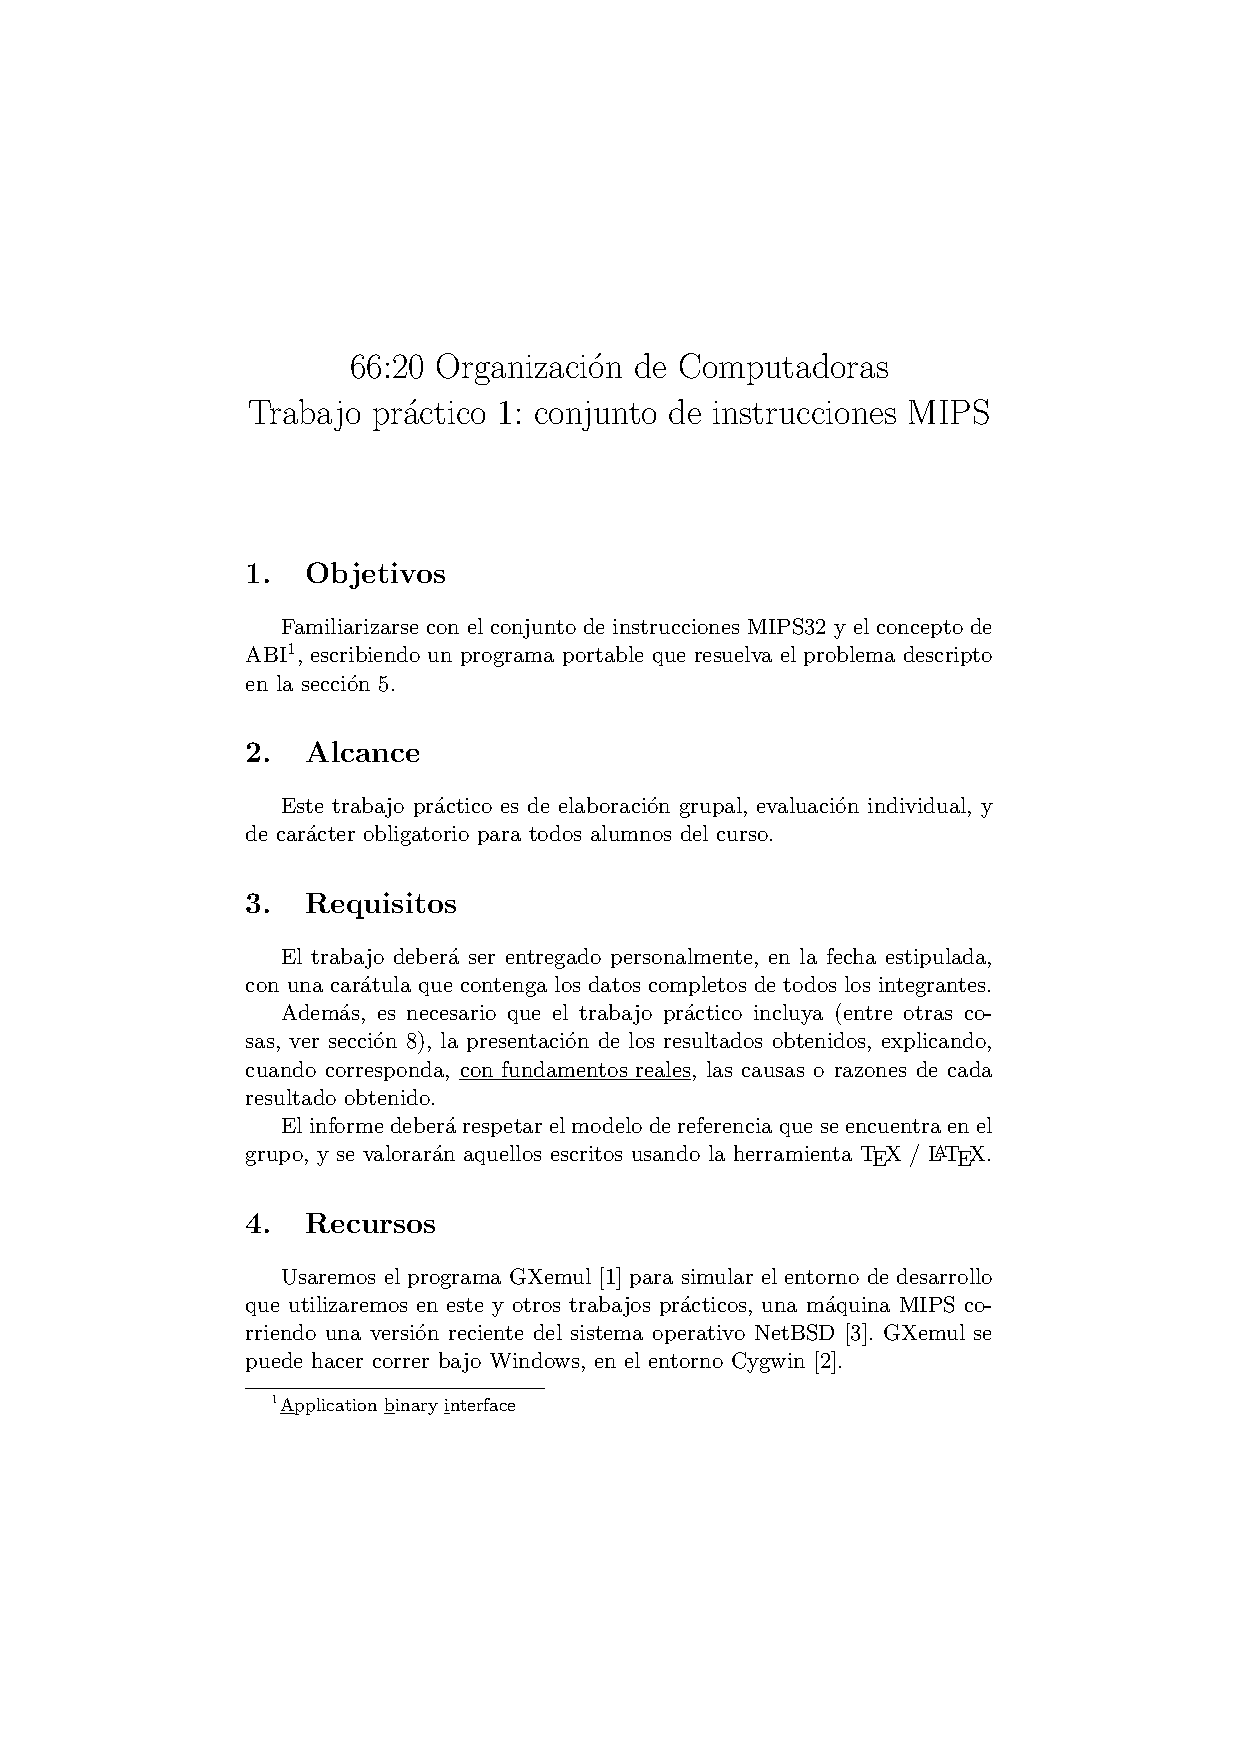
\includegraphics[scale=1, page = 1, clip, trim=20mm 36mm 20mm 35mm]{files/enunciado.pdf}
	\end{figure}
	
	\newpage
	\begin{figure}[H]
		\centering
		\includegraphics[scale=1, page = 2, clip, trim=20mm 36mm 20mm 20mm]{files/enunciado.pdf}
	\end{figure}
	
	\newpage
	\begin{figure}[H]
		\centering
		\includegraphics[scale=1, page = 3, clip, trim=20mm 36mm 20mm 20mm]{files/enunciado.pdf}
	\end{figure}
	
	\newpage
	\begin{figure}[H]
		\centering
		\includegraphics[scale=1, page = 4, clip, trim=20mm 36mm 20mm 20mm]{files/enunciado.pdf}
	\end{figure}
	
	\newpage
	\begin{figure}[H]
		\centering
		\includegraphics[scale=1, page = 5, clip, trim=20mm 36mm 20mm 20mm]{files/enunciado.pdf}
	\end{figure}
	
	\section{Desarrollo}
	
		El programa puede tomar opciones de entrada para indicar el tipo de ordenamiento (alfabético o numérico) y argumentos que designan la salida y el archivo a ordenar.
		
	\subsection{Implementación}
		
		Los errores se definen como cadenas de caracteres constantes. Los mensajes de error se llaman con una función a la que se le pasa el mensaje a mostrar y el número que le corresponde al error.
		
		Las invocaciones a la línea de comandos (como el pedido de versión o de ayuda) también se guardan en cadenas. El tipo de mensaje a mostrar es pasado a la función que los visualiza.
		
		El Quicksort diferencia el tipo de ordenamiento que se hará en un método de ordenamiento general. Esto se logra con un entero identificador: si vale 1, el ordenamiento es numérico; para cualquier otro valor se realizará un ordenamiento alfabético. En el primer caso se utilizará una función atoi para pasar las cadenas de caracteres a números enteros. En el otro caso se compararán las cadenas entre sí.
		
		Al inicio de la función \texttt{main} se verifican los argumentos ingresados para ver si coinciden con las opciones requeridas.	Así se puede responder de acuerdo con el comportamiento elegido. 
		
	\subsection{Pruebas}
	
	\subsubsection{Entradas incorrectas}
	Ingresando sólo el nombre del programa ejecutable:
	\begin{verbatim}
$ qsort
qsort: La cantidad de parametros no es la correcta.
Intente 'qsort -h' para mas informacion
	\end{verbatim}
	
	Ingresando un argumento inválido:
	\begin{verbatim}
$ qsort -w
qsort: La combinacion de parametros no es la correcta.
Intente 'qsort -h' para mas informacion
	\end{verbatim}
	
	Ingresando un argumento inválido en ordenamiento alfabético (\texttt{+} en lugar de \texttt{-}):
	\begin{verbatim}
$ qsort -o + zeta.txt
qsort: La combinacion de parametros no es la correcta.
Intente 'qsort -h' para mas informacion
	\end{verbatim}
	
	Ingresando un argumento inválido en ordenamiento numérico (\texttt{g} en lugar de \texttt{-}):
	\begin{verbatim}
$ qsort -n -o g zeta.txt
qsort: La combinacion de parametros no es la correcta.
Intente 'qsort -h' para mas informacion
	\end{verbatim}
	
	Ingresando más argumentos de los necesarios:
	\begin{verbatim}
$ qsort f f f f f
qsort: La cantidad de parametros no es la correcta.
Intente 'qsort -h' para mas informacion
	\end{verbatim}
	
	Ingresando un archivo que no existe:
	\begin{verbatim}
$ qsort -o - numbers.txt
El archivo que quiere ordenar no existe
	\end{verbatim}
	
	Ingresando el orden incorrecto de parámetros (primero \texttt{-o} y luego \texttt{-n}):
	\begin{verbatim}
$ qsort -o -n - numeros.txt
qsort: La combinacion de parametros no es la correcta.
Intente 'qsort -h' para mas informacion
	\end{verbatim}
	
	
	
	\subsubsection{Ordenando líneas}
	Ingresando un archivo para ordenar alfabéticamente:
	\begin{verbatim}
$ qsort -o - zeta.txt
zzzzzzzzzzzz a
zzzzzzzzzzzz b
zzzzzzzzzzzz sabia que Asuntos Internos le tendia una trampa
	\end{verbatim}
	
	\begin{verbatim}
$ qsort -o - numeros.txt
1
10
2
3
4
5
6
7
8
9
	\end{verbatim}
	
	Ingresando un archivo para ordenar numéricamente:
	\begin{verbatim}
$ qsort -n -o - zeta.txt
zzzzzzzzzzzz b
zzzzzzzzzzzz sabia que Asuntos Internos le tendia una trampa
zzzzzzzzzzzz a
	\end{verbatim}
	
	\begin{verbatim}
$ qsort -n -o - numeros.txt
1
2
3
4
5
6
7
8
9
10
	\end{verbatim}

	\subsection{Diagramas de stack}
	
	\begin{figure}[H]
		\centering
		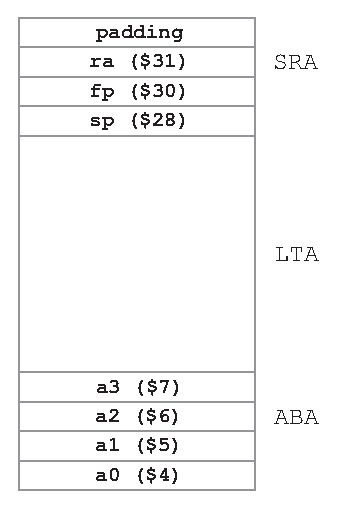
\includegraphics[scale=1]{files/stack_frame.eps}
		\caption{Diagrama de stack para...}
		\label{fig:diag:stack}
	\end{figure}
	\section{Conclusiones}
	
	\newpage
	\section{Código fuente}
	
	\begin{lstlisting}
#include <stdio.h>
#include <string.h>
#include <stdlib.h>
#include <stdbool.h>

#define salida_error_parametros 1
#define salida_error_archivo_inexistente 2
#define mensaje_error_cantidad_parametros "qsort: La cantidad de parametros no es la correcta.\nIntente 'qsort -h' para mas informacion"
#define mensaje_error_parametros "qsort: La combinacion de parametros no es valida.\nIntente 'qsort -h' para mas informacion"
#define mensaje_error_archivo_inexistente "El archivo que quiere ordenar no existe"
#define MENSAJE_AYUDA "Usage:\n\tqsort -h\n\tqsort -V\n\tqsort [options] archivo\nOptions:\n\t-h, --help \tImprime ayuda.\n\t-V, --version \tVersion del programa.\n\t-o, --output \tArchivo de salida.\n\t-n, --numeric \tOrdenar los datos numericamente en vez de alfabeticamente.\nExamples:\n\tqsort -n numeros.txt"
#define VERSION "v1.0"
	\end{lstlisting}
	
	\begin{lstlisting}
void mostrar_error_y_salir(char *mensaje_error, int numero_salida){
	fprintf(stderr, "%s\n", mensaje_error);
    exit(numero_salida);
}
	\end{lstlisting}
	
	\begin{lstlisting}
void mostrar_version(){printf("%s\n", VERSION);}
	\end{lstlisting}
	
	\begin{lstlisting}
void mostrar_ayuda(){printf("%s\n", MENSAJE_AYUDA);}
	\end{lstlisting}
	
	\begin{lstlisting}
int obtener_longitud_maxima(FILE* archivo){
    // Obtiene longitud contando el \n o \0 del final
    // ejemplo: para "hola", maximo = 5
    int maximo = 0;
    int actual = 0;
    int caracter;
    while ((caracter = fgetc(archivo)) != EOF){
        actual++;
        if (caracter == '\n'){
            if (actual > maximo) maximo = actual;
            actual = 0;
        }
    }
    return maximo;
}
	\end{lstlisting}
	
	\begin{lstlisting}
int obtener_cantidad_palabras(FILE *archivo, int len){
    int cantidad = 0;
    char c = ' ';
    while (c != EOF){
        c = fgetc(archivo);
        if (c == '\n') cantidad ++;
    }
    //printf("%i\n", cantidad);
    return cantidad;
}
	\end{lstlisting}
	
	\begin{lstlisting}
void obtener_palabras(FILE* archivo, char **lista_palabras, int len, int cantidad_palabras){
    int indice = 0;
    char palabra[len + 1];

    for (int i = 0; i < cantidad_palabras; i++){
        fgets(palabra, len + 1, archivo);
        for(int j = 0; j < (strlen(palabra) + 1); j++){
            if (palabra[j] == '\n' || palabra[j] == EOF) palabra[j] = '\0';
        }
        lista_palabras[indice] = malloc(strlen(palabra) + 1);
        strcpy(lista_palabras[indice], palabra);
        indice ++;
    }
}
	\end{lstlisting}
	
	\begin{lstlisting}
int comparar_como_numero(const char *numero1,const char *numero2){
    int n1 = atoi(numero1);
    int n2 = atoi(numero2);
    return(n1-n2);
}
	\end{lstlisting}
	
	\begin{lstlisting}
void orgaqsortgeneral(char** izq, char** der, int (*fcmp)(const char *,const char *)){
    if (izq <= der) {
        char *aux;
        char **inicio = izq;
        char **fin = der;
        while (inicio < fin){
            while ((fcmp(*inicio, *izq) <= 0) && (inicio < der))inicio++;
            while ((fcmp(*fin, *izq) > 0) && (fin > izq)) fin--;
            if (inicio < fin){
                aux = *inicio;
                *inicio = *fin;
                *fin = aux;
            }
        }
        aux = *izq;
        *izq = *fin;
        *fin = aux;
        orgaqsortgeneral(izq, fin-1, fcmp);
        orgaqsortgeneral(fin+1, der, fcmp);
    }
}
	\end{lstlisting}
	
	\begin{lstlisting}
void orgaqsort(char **izq, char **der, int num){
    //Si num = 0 ordena alfabeticamente
    //Si num != 0 ordena como numeros
    if (num) orgaqsortgeneral(izq, der, comparar_como_numero);
    else orgaqsortgeneral(izq, der, strcmp);
}
	\end{lstlisting}
	
	\begin{lstlisting}
int main(int argc, char *argv[]){

    int longitud, cantidad_palabras, nro_archivo_entrada, nro_archivo_salida, criterio_ordenamiento;
    char** lista_palabras;
    FILE* archivo;
    FILE* output = stdout;

    if ((argc < 2) || argc > 5) {
        mostrar_error_y_salir(mensaje_error_cantidad_parametros, salida_error_parametros);
    }

    else if ((strcmp(argv[1], "-h") == 0) || (strcmp(argv[1], "--help") == 0)){
        if(argc != 2) mostrar_error_y_salir(mensaje_error_cantidad_parametros, salida_error_parametros);
        mostrar_ayuda();
        return 0;
    }
    else if ((strcmp(argv[1], "-V") == 0) || (strcmp(argv[1], "--version") == 0)){
        if(argc != 2) mostrar_error_y_salir(mensaje_error_cantidad_parametros, salida_error_parametros);
        mostrar_version();
        return 0;
    }

    else if ((strcmp(argv[1], "-o") == 0) || (strcmp(argv[1], "--output") == 0)){
        if (argc != 4) mostrar_error_y_salir(mensaje_error_cantidad_parametros, salida_error_parametros);
        nro_archivo_entrada = 3;
        nro_archivo_salida = 2;
        criterio_ordenamiento = 0;
    }

    else if ((argc > 2) && ((strcmp(argv[2], "-o") == 0) || (strcmp(argv[2], "--output") == 0)) && ((strcmp(argv[1], "-n") == 0) || (strcmp(argv[1], "--numeric") == 0))) {
        if (argc != 5) mostrar_error_y_salir(mensaje_error_cantidad_parametros, salida_error_parametros);
        nro_archivo_entrada = 4;
        nro_archivo_salida = 3;
        criterio_ordenamiento = 1;
    }

    else mostrar_error_y_salir(mensaje_error_parametros, salida_error_parametros);

    archivo = fopen(argv[nro_archivo_entrada],"r");
    if (!archivo) mostrar_error_y_salir(mensaje_error_archivo_inexistente, salida_error_archivo_inexistente);
    if (strcmp(argv[nro_archivo_salida], "-")){
        output = fopen(argv[nro_archivo_salida], "w");
        if (!output) mostrar_error_y_salir(mensaje_error_archivo_inexistente, salida_error_archivo_inexistente);
    }

    longitud = obtener_longitud_maxima(archivo);
    rewind(archivo);
    cantidad_palabras = obtener_cantidad_palabras(archivo, longitud);
    rewind(archivo);
    lista_palabras = malloc(cantidad_palabras * sizeof(char*));
    obtener_palabras(archivo, lista_palabras, longitud, cantidad_palabras);
    orgaqsort(lista_palabras, lista_palabras + cantidad_palabras -1, criterio_ordenamiento);
    for (int i = 0; i < cantidad_palabras; i++){
        fprintf(output, "%s\n",lista_palabras[i]);
        free(lista_palabras[i]);
    }
    fclose(archivo);
    fclose(output);
    free(lista_palabras);
    return 0;
}
	\end{lstlisting}

\end{document}
